\documentclass[compress, 10pt]{beamer}
\usepackage{nuaabeamer}

\usepackage{graphics}

\usepackage{frame}
\usepackage{pgf}
\usepackage[UTF8, noindent]{ctex}
\usepackage{times}
\usepackage{amsmath}
\usepackage{algorithm}
\usepackage[noend]{algpseudocode}
\usefonttheme{professionalfonts}
\usepackage{listings}
\usepackage{color}
\usepackage{xcolor}
\lstset{
    language=C++,
    basicstyle=\tt,
    keywordstyle=\color{purple}\bfseries,
    identifierstyle=\color{brown!80!black},
    commentstyle=\color{gray}
    showstringspaces=false,
    % tiny font
    % basicstyle=\tiny,
    numbers=left,
    breaklines=true,
}

\usepackage{caption}
\setbeamertemplate{caption}[numbered]{}

\usepackage[backend=bibtex,style=ieee,sorting=none]{biblatex}
% \addbibresource{ref.bib}
\setbeamerfont{footnote}{size=\tiny}

\usepackage{subfigure}

\makeatletter
\let\@@magyar@captionfix\relax
\makeatother

\newcommand{\Title}{SPH方法调研与汇报一}
\newcommand{\Reporter}{包晨宇}
\newcommand{\Instructor}{吕宏强}
\newcommand{\Institute}{南京航空航天大学}

\begin{document}

\captionsetup[figure]{font=footnotesize,labelfont=footnotesize}

\title{\Title}
\author{汇报人:\Reporter \\ \vspace{1em} 指导人:\Instructor}
\date{\today}
\institute{\Institute}

\begin{frame}
    \begin{figure}[H]
        \centering
        
\includegraphics[width=0.2\textwidth]{logo.pdf}
    \end{figure}
    \maketitle
\end{frame}

\section*{目录}
\begin{frame}
    \frametitle{\secname}
    \tableofcontents[sections={<1-5>}]
\end{frame}

\AtBeginSection[] {%在每一节前面加入目录显示当前节的目录结构
	\begin{frame}
		\frametitle{目录}
		\tableofcontents[currentsection,currentsubsection,hideothersubsections,sectionstyle=show/shaded,]
		\addtocounter{framenumber}{-1}  %目录页不计入页码
	\end{frame}
}


\section{进度简介}

\begin{frame}
    \begin{block}{公式查询及推导进度}
        查询了 WCSPH 相关公式以及核函数插值方法,并推导了相关导数公式,
        以及控制方程的离散形式
    \end{block}
    \begin{block}{CPP 求解器程序实现进度}
        \begin{itemize}
            \item 多个核函数及其导数模块实现
            \item 粒子结构体以及粒子与粒子作用函数实现
            \item 求解器主程序框架实现
            \item 后处理输出(暂时以 XML 格式输出,用 pyvista 处理)
        \end{itemize}
    \end{block}
\end{frame}
\section{公式查询及推导进度}

\subsection{核函数插值的公式推导}

\begin{frame}
    \frametitle{插值核函数的一般形式}
Usually, kernel function has the form of:

\begin{equation}
    W(\vec{r})=W\left(
        \frac{r}{h}
    \right)=W(q)
\end{equation}

where:

\begin{equation}
    \begin{aligned}
        q &= \frac{r}{h} \quad &\Rightarrow \quad \frac{dq}{dr}= \frac{1}{h}\\
        r &= \sqrt{\sum_{k=1}^d x_k^2} \quad &\Rightarrow \quad \frac{\partial r}{\partial x_k} = \frac{x_k}{r}\\
    \end{aligned}
\end{equation}
\end{frame}


\begin{frame}
    \frametitle{插值核函数的梯度}
    \begin{equation}
        \begin{aligned}
            \frac{\partial W}{\partial x_k} &= \frac{\partial W}{\partial q}\frac{\partial q}{\partial x_k}\\
            &= \frac{\partial W}{\partial q}\frac{\partial q}{\partial r}\frac{\partial r}{\partial x_k}\\
            &= \frac{\partial W}{\partial q}\frac{1}{h}\frac{x_k}{r}\\
            &= \frac{1}{h}\frac{x_k}{r}\frac{\partial W}{\partial q}\\
            &= \frac{1}{h}\frac{x_k}{r}W^\prime
        \end{aligned}
    \end{equation}
    thus it's obvious that:
    \begin{equation}
        \nabla W = \frac{1}{h}\frac{\vec{r}}{r}W^\prime
        ,\quad |\nabla W| = \frac{1}{h}|W^\prime|
    \end{equation}
\end{frame}


\begin{frame}
    \frametitle{插值核函数的拉普拉斯算子值}
    
\begin{equation}
    \begin{aligned}
        \frac{\partial^2 W}{\partial x_k^2} &= \frac{\partial}{\partial x_k}\left(
            \frac{1}{h}\frac{x_k}{r}W^\prime
        \right)\\
        &= \frac{1}{h}W^\prime \left(
            \frac{1}{r} - \frac{x_k^2}{r^3}
        \right)+
        \frac{1}{h}\frac{x_k}{r}\frac{\partial W^\prime}{\partial x_k}\\
        &= \frac{1}{h}W^\prime \frac{r^2-x_k^2}{r^3}+
        \frac{x_k}{hr} \frac{\partial W^\prime}{\partial q}\frac{\partial q}{\partial r}\frac{\partial r}{\partial x_k}\\
        &= \frac{1}{h}W^\prime \frac{r^2-x_k^2}{r^3}+
        \frac{x_k}{hr} \frac{\partial W^\prime}{\partial q}\frac{1}{h}\frac{x_k}{r}\\
        &= \frac{1}{h}W^\prime \frac{r^2-x_k^2}{r^3}+
        \frac{1}{h^2r^2}x_k^2 W^{\prime\prime}\\
        &= \frac{1}{h}W^\prime \frac{r^2-x_k^2}{r^3}+
        \frac{x_k^2}{h^2r^2} W^{\prime\prime}
    \end{aligned}
\end{equation}
\end{frame}


\begin{frame}
    \frametitle{插值核函数的拉普拉斯算子值}
    \begin{equation}
        \nabla^2 W = \sum_{k=1}^d \frac{\partial^2 W}{\partial x_k^2} = 
            \frac{d-1}{hr}W^\prime + \frac{1}{h^2}W^{\prime\prime}
    \end{equation}
    
    when $r\to 0$, we have:
    
    \begin{equation}
        \nabla^2 W = \lim_{r/h\to 0} \nabla^2 W = \frac{d}{h^2}W^{\prime\prime}
    \end{equation}
\end{frame}

\subsection{核函数插值格式}

\begin{frame}
    \frametitle{梯度的核函数插值格式}
    From the property shared with $\delta$ function:

\begin{equation}
    A(\vec{r}) = 
    \int_{\Omega} A(\vec{r}^\prime) 
    W(\vec{r} - \vec{r}^\prime) \mathrm{d}\vec{r}^\prime
\end{equation}

In particle discretization, we have:

\begin{equation}
    A_i = \sum_{j} \frac{m_j}{\rho_j} A_j W_{ij}
\end{equation}

where:

\begin{equation}
    W_{ij} = W(\vec{r}_i - \vec{r}_j)\quad \text{and} 
    \quad \sum_{j} \frac{m_j}{\rho_j} W_{ij} = 1
\end{equation}

This provides a way to interpolate the value of $A$ at any point $\vec{r}$.
\end{frame}

\begin{frame}
    \frametitle{梯度的核函数插值格式}
    Consider a scalar function $A(\vec{r})$ distributed in space $\mathbb{R}^\text{dim}$. 
Let's see $\nabla A(\vec{r})$:
\begin{equation}
    \begin{aligned}
        \nabla A(\vec{r}) 
        &= \int_{\Omega} \nabla A(\vec{r}^\prime) W(\vec{r} - \vec{r}^\prime) \mathrm{d}\vec{r}^\prime \\
        &= \int_{\Omega} \nabla A(\vec{r}^\prime) W(\vec{r}^\prime - \vec{r}) \mathrm{d}\vec{r}^\prime \\
        &= \int_{\partial \Omega} A(\vec{r}^\prime) \vec{n} W(\vec{r}^\prime - \vec{r}) \mathrm{d}S^\prime
        -\int_{\Omega} A(\vec{r}^\prime) \nabla W(\vec{r}^\prime - \vec{r}) \mathrm{d}\vec{r}^\prime\\
        &= \int_{\Omega} A(\vec{r}^\prime) \nabla W(\vec{r} - \vec{r}^\prime) \mathrm{d}\vec{r}^\prime
    \end{aligned}
\end{equation}

The above formula use property of compactness and symmetry of kernel function. 
In particle discretization, we have:

\begin{equation}
    \nabla A_i = \sum_{j} \frac{m_j}{\rho_j} A_j \nabla W_{ij}
\end{equation}
\end{frame}

\begin{frame}
    \frametitle{梯度的核函数插值格式}
    where:

\begin{equation}
    \nabla W_{ij} = \nabla W(\vec{r}_i - \vec{r}_j)
\end{equation}

However, according to 'Smoothed Particle Hydrodynamic' from Monaghan 1992, 
such form of 1-st derivative interpolation is not accurate enough. 
He proposed a better way to do such interpolation. 
Supposing we have a scalar called $\phi$, let's consider $\phi\nabla A$ 's approximation:

\begin{equation}
    \begin{aligned}
        \phi\nabla A = \nabla(\phi A) - A\nabla\phi
    \end{aligned}
\end{equation}
\end{frame}

\begin{frame}
    \frametitle{梯度的核函数插值格式}

    Use interpolation above, we have:
\begin{equation}
    \begin{aligned}
        \phi_i (\nabla A)_i &= 
            \sum_j \frac{m_j}{\rho_j} \phi_j A_j \nabla W_{ij} -
            A_i\sum_j \frac{m_j}{\rho_j}  \phi_j \nabla W_{ij}\\
            &= \sum_j \frac{m_j}{\rho_j} \phi_j( A_j-A_i) \nabla W_{ij}
    \end{aligned}
\end{equation}

thus we have:

\begin{equation}
    (\nabla A)_i = \frac{1}{\phi_i}\sum_j \frac{m_j}{\rho_j} \phi_j( A_j-A_i) \nabla W_{ij} 
\end{equation}

\end{frame}

\begin{frame}
    \frametitle{梯度的核函数插值格式}

    noting that $A_{ij} = A_i - A_j$, we have:

\begin{equation}
    (\nabla A)_i = -\frac{1}{\phi_i}\sum_j \frac{m_j}{\rho_j}\phi_j A_{ij} \nabla W_{ij}
\end{equation}

For example, when we focus on $\frac{1}{\rho}\nabla p$, 
we have 2 ways to obtain its value:
\begin{equation}
    \begin{aligned}
        \phi = 1 \quad &\Rightarrow \quad 
            (\nabla p)_i = \sum_j \frac{m_j}{\rho_j} (p_j-p_i) \nabla W_{ij} \\
        \phi_i = \frac{1}{\rho} \quad &\Rightarrow \quad 
            \frac{1}{\rho}\nabla p = \nabla \left(
                \frac{p}{\rho}
            \right)+
            \frac{p}{\rho^2}\nabla \rho\\
            &\Rightarrow\quad
            \left(\frac{\nabla p}{\rho}\right)_i=
            \sum_j m_j \left(
                \frac{p_j}{\rho_j^2}+\frac{p_i}{\rho_i^2}
            \right) \nabla W_{ij}
    \end{aligned}
\end{equation}

当我推导到这里的时候,就感觉到这个数值格式似乎存在一些问题。

\end{frame}

\begin{frame}
    \frametitle{散度的核函数插值格式}
    Now let's consider a vector $\vec{A}$ distributed in space $\mathbb{R}^\text{dim}$.
    Let's see $\nabla\cdot\vec{A}$:
    \begin{equation}
        \begin{aligned}
            \nabla\cdot\vec{A}(\vec{r}) &= \int_{\Omega} \nabla\cdot\vec{A}(\vec{r}^\prime) W(\vec{r} - \vec{r}^\prime) \mathrm{d}\vec{r}^\prime \\
            &= \int_{\Omega} \nabla\cdot\vec{A}(\vec{r}^\prime) W(\vec{r}^\prime - \vec{r}) \mathrm{d}\vec{r}^\prime \\
            &= \int_{\partial \Omega} \vec{A}(\vec{r}^\prime) \cdot \vec{n} W(\vec{r}^\prime - \vec{r}) \mathrm{d}S^\prime -
            \int_{\Omega} \vec{A}(\vec{r}^\prime) \cdot \nabla W(\vec{r}^\prime - \vec{r}) \mathrm{d}\vec{r}^\prime\\
            &= \int_{\Omega} \vec{A}(\vec{r}^\prime) \cdot \nabla W(\vec{r} - \vec{r}^\prime) \mathrm{d}\vec{r}^\prime
        \end{aligned}
    \end{equation}
    
    In particle discretization, we have:
    
    \begin{equation}
        (\nabla\cdot\vec{A})_i = \sum_{j} \frac{m_j}{\rho_j} \vec{A}_j \cdot \nabla W_{ij}
    \end{equation}
    
\end{frame}

\begin{frame}
    \frametitle{散度的核函数插值格式}
    where:

\begin{equation}
    \nabla W_{ij} = \nabla W(\vec{r}_i - \vec{r}_j)
\end{equation}

However, this way o interpolation is not accurate enough. 
Let's consider a scalar $\phi$ here:

\begin{equation}
    \phi \nabla\cdot \vec{A} = \nabla\cdot(\phi \vec{A}) - \vec{A}\cdot\nabla\phi
\end{equation}

Use interpolation above, we have:

\begin{equation}
    \begin{aligned}
        \phi_i (\nabla\cdot \vec{A})_i &= 
            \sum_j \frac{m_j}{\rho_j} \phi_j \vec{A}_j \cdot \nabla W_{ij} -
            \vec{A}_i\cdot\sum_j \frac{m_j}{\rho_j}  \phi_j \nabla W_{ij}\\
            &=
            \sum_j \frac{m_j}{\rho_j} \phi_j (\vec{A}_j-\vec{A}_i) \cdot \nabla W_{ij}\\
            &=
            -\sum_j \frac{m_j}{\rho_j} \phi_j \vec{A}_{ij} \cdot \nabla W_{ij}
    \end{aligned}
\end{equation}
\end{frame}

\begin{frame}
    \frametitle{散度的核函数插值格式}
    where $\vec{A}_{ij} = \vec{A}_i - \vec{A}_j$. 
For example, when we calculate $\rho \nabla\cdot\vec{v}$, interpolation above reveals:

\begin{equation}
    (\rho \nabla\cdot \vec{v})_i = -\sum_j m_j \vec{v}_{ij} \cdot \nabla W_{ij}
\end{equation}

such interpolation is widely used in SPH method.
\end{frame}

\begin{frame}
    \frametitle{拉普拉斯算子的核函数插值格式}
    Now let's consider a scalar function $A(\vec{r})$ distributed in space $\mathbb{R}^\text{dim}$.
\begin{equation}
    \begin{aligned}
        \nabla^2 A(\vec{r}) &= \int_{\Omega} \nabla^2 A(\vec{r}^\prime) W(\vec{r} - \vec{r}^\prime) \mathrm{d}\vec{r}^\prime \\
        &= \int_{\Omega} \nabla^2 A(\vec{r}^\prime) W(\vec{r}^\prime - \vec{r}) \mathrm{d}\vec{r}^\prime \\
        &= \int_{\partial \Omega} \nabla A(\vec{r}^\prime) \cdot \vec{n} W(\vec{r}^\prime - \vec{r}) \mathrm{d}S^\prime -
        \int_{\Omega} \nabla A(\vec{r}^\prime) \cdot \nabla W(\vec{r}^\prime - \vec{r}) \mathrm{d}\vec{r}^\prime\\
        &= -\int_{\Omega} \nabla A(\vec{r}^\prime) \cdot \nabla W(\vec{r}^\prime - \vec{r}) \mathrm{d}\vec{r}^\prime\\
        &= -\int_{\partial \Omega} A(\vec{r}^\prime)\vec{n} \cdot \nabla W(\vec{r}^\prime - \vec{r}) \mathrm{d}S^\prime +
        \int_{\Omega} A(\vec{r}^\prime) \nabla^2 W(\vec{r}^\prime - \vec{r}) \mathrm{d}\vec{r}^\prime\\
        &= \int_{\Omega} A(\vec{r}^\prime) \nabla^2 W(\vec{r} - \vec{r}^\prime) \mathrm{d}\vec{r}^\prime
    \end{aligned}
\end{equation}
\end{frame}

\begin{frame}
    \frametitle{拉普拉斯算子的核函数插值格式}
    The same problem with this formula is accuracy. 
For this part, 
I consult a large number of references, 
but each reference has its own way of interpolation.

in 1985, Brookshaw proposed a way based on Taylor expansion:

\begin{equation}
    (\nabla^2 A)_i = -\sum_{j} \frac{m_j}{\rho_j} A_{ij}\frac{2|\nabla W_{ij}|}{|r_{ij}|}
\end{equation}

However, after I reading the original paper, I find he only proposed a 1-D case's formula, 
In Dan Koschier's paper, he directly use the above formula in 3-D case. 
And in another paper from Price, 2012, he use the following formula:

\begin{equation}
    (\nabla^2 A)_i = 2\sum_{j} \frac{m_j}{\rho_j} A_{ij}\frac{|\nabla W_{ij}|}{|r_{ij}|}
\end{equation}
\end{frame}

\begin{frame}
    \frametitle{拉普拉斯算子的核函数插值格式}

    My math is not good enough to prove the correctness of this formula. 
But from my personal formula, I think the following formula is more reasonable:

\begin{equation}
    \begin{aligned}
        \nabla^2 A(\vec{r})&= 
        \int_{\Omega} \nabla A(\vec{r}^\prime) \cdot \nabla W(\vec{r}- \vec{r}^\prime ) \mathrm{d}\vec{r}^\prime\\
        &\approx
        \sum_j \frac{m_j}{\rho_j} \frac{A_i-A_j}{|\vec{r}_i-\vec{r}_j|^2}
        (\vec{r}_i - \vec{r}_j)\cdot \nabla W_{ij}\\
        &=\sum_j \frac{m_j}{\rho_j}\frac{A_{ij}}{r_{ij}^2}\vec{r}_{ij}\cdot \nabla W_{ij}
    \end{aligned}
\end{equation}

From the above formula, $|\nabla W_{ij}|$ shares the same direction with $\vec{r}_{ij}$,
thus we have:

\begin{equation}
    \nabla^2 A(\vec{r})\approx
    \sum_j \frac{m_j}{\rho_j}\frac{A_{ij}}{r_{ij}}|\nabla W_{ij}|
\end{equation}

\end{frame}

\begin{frame}
    \frametitle{拉普拉斯算子的核函数插值格式}

    this result is quite similar to Price, 2012's formula except for the coefficient '$2$'.
Currently, I have no idea on why there is a '$2$' in his formula. 
A possible explanation is that it comes from the Taylor expansion of $W$.

\end{frame}

\begin{frame}
    \frametitle{向量的拉普拉斯算子的核函数插值格式}

    I copy this from Price, 2012's paper but really have no idea on how to prove it:

\begin{equation}
    \begin{aligned}
        (\nabla^2 \vec{A})_i&=-2\sum_j \frac{m_j}{\rho_j}\vec{A}_{ij}\frac{|\nabla W_{ij}|}{r_{ij}}\\
    \end{aligned}
\end{equation}

What's more, for a divergence-free vector field $\vec{A}$ (which has $\nabla\cdot\vec{A}=0$), 
Price proposed a way to calculate $\nabla^2 \vec{A}$:

\begin{equation}
    (\nabla^2 \vec{A})_i=2(d+2)\sum_{j} 
    \frac{m_j}{\rho _j} \frac{\vec{A}_{ij}\cdot \vec{r}_{ij}}{r_{ij}^2}\nabla W_{ij}
\end{equation}

For weak compressible SPH method, this scheme also works.

\end{frame}
\section{CPP 求解器程序实现进度}

\subsection{弱可压 WCSPH 控制方程}

\begin{frame}
    This method allows density to vary in space, instead of keeping it constant. 
This method is widely used in SPH method.

The governing equation is as follows (Lagrange form):

\begin{equation}
    \begin{aligned}
        \frac{\mathrm{d} \rho}{\mathrm{d} t} &= -\rho \nabla\cdot \vec{v}\\
        \frac{\mathrm{d} \vec{v}}{\mathrm{d} t} &= -\frac{1}{\rho}\nabla p + \vec{g} + \nu \nabla^2 \vec{v}\\
        \frac{\mathrm{d} \vec{r}}{\mathrm{d} t} &= \vec{v}\\
        \frac{\mathrm{d}p}{\mathrm{d} \rho} &= c^2
    \end{aligned}
\end{equation}

WCSPH allows density to vary in space, thus pressure without $p_0$ can be written as:

\begin{equation}
    p = c^2(\rho - \rho_0)
\end{equation}
\end{frame}

\begin{frame}
    Here for initializing the whole fluid system, 
we need to calculate the initial pressure $p$ and density $\rho$.
Usually, pressure obeys the stable hydrostatic equation:

\begin{equation}
    p = \rho g h+ p_0
\end{equation}

In calculation, we can set $p_0=0$ for convenience. 
And density can be calculated from the following equation:

\begin{equation}
    \rho = \rho_0 + \frac{p}{c^2}
\end{equation}

For $c$ in water is $1481m/s$, $\Delta\rho$ would be small.
\end{frame}

\begin{frame}
    Thus a whole fluid solver is proposed as follows:

\begin{algorithm}[H]
    \caption{WCSPH Simple Solver}
    \begin{algorithmic}[1]
        \State \textbf{Input:} $\rho_0, c, \nu, \vec{g}, \Delta t$ etc.
        \State \textbf{Output:} $\rho, \vec{v}, p$
        \State \textbf{Initialize:}:
        $p = \rho_0 g h, \rho = \rho_0 + \frac{p}{c^2}, \vec{v} = \vec{v}_0$
        \While{current time step < total time step}
            \For{each particle $i$}
                \State Update $\rho$ using $\frac{d\rho}{dt}= -\rho \nabla\cdot \vec{v}$
            \EndFor
            \For{each particle $i$}
                \State Update $\vec{v}$ to $\vec{v}^*$ without pressure using $\frac{d\vec{v}}{dt}= \vec{g} + \nu \nabla^2 \vec{v}$
            \EndFor
            \For{each particle $i$}
                \State Update $p$ using $p = c^2(\rho - \rho_0)$
            \EndFor
            \For{each particle $i$}
                \State Update $\vec{v}$ to $\vec{v}^{n+1}$ with pressure using $\frac{d\vec{v}}{dt}= -\frac{1}{\rho}\nabla p$
                \State Update $\vec{r}$ using $\frac{d\vec{r}}{dt}= \vec{v}$
            \EndFor
        \EndWhile
    \end{algorithmic}
\end{algorithm}
\end{frame}

\subsection{SPH 离散格式}

\begin{frame}
    \begin{equation}
        \left(\frac{d\rho}{dt}\right)_i = 
        \sum_j m_j (\vec{v}_i-\vec{v}_j)\cdot \nabla W_{ij}
    \end{equation}
    
    here we obtain the density of each particle at the next time step:
    
    \begin{equation}
        \rho_i^{n+1} = \rho_i^n + \Delta t \sum_j m_j (\vec{v}_i-\vec{v}_j)\cdot \nabla W_{ij}
    \end{equation}
    
    However, this step ususally needs correction (accoring to SmoothedParticles.jl):
    
    \begin{equation}
        \left(\frac{d\rho}{dt}\right)_i = 
        \sum_j m_j (\vec{v}_i-\vec{v}_j)\cdot \nabla W_{ij}+
        2\epsilon_\rho\sum_j m_j (\rho_i-\rho_j)\frac{|\nabla W_{ij}|}{r_{ij}}
    \end{equation}
    
    here $\epsilon_\rho$ is $1\times 10^{-6}$.
\end{frame}

\begin{frame}
    \begin{equation}
        \frac{d\vec{v}}{dt} = -\frac{1}{\rho}\nabla p+\vec{g} + \frac{\mu}{\rho} \nabla^2 \vec{v}
    \end{equation}
    
    Here we use the following formula to calculate $\nabla^2 \vec{v}$:
    
    \begin{equation}
        \nabla^2 \vec{v} = 2(d+2)\sum_j
        \frac{m_j}{\rho_j}\frac{\vec{v}_{ij}\cdot \vec{r}_{ij}}{r_{ij}^2}\nabla W_{ij}
    \end{equation}
    
    To avoid singularity, we modify the above formula as follows:
    
    \begin{equation}
        \nabla^2 \vec{v} = 2(d+2)\sum_j
        \frac{m_j}{\rho_j}\frac{\vec{v}_{ij}\cdot \vec{r}_{ij}}{r_{ij}^2+0.01h^2}\nabla W_{ij}
    \end{equation}
    
    Actucally, after reading Price's formula and Koschier's reference and Delong Xu's 
    form, I'm confused this part has no unified form. I simply apply current formula
    
    \begin{equation}
        \vec{f}_{\text{vis}}=
        \mu \sum_{j} m_j \frac{2(d+2)}{\rho_i\rho_j}
        \frac{\vec{v}_{ij}\cdot \vec{r}_{ij}}{r_{ij}^2+0.01h^2}\nabla W_{ij}
    \end{equation}
\end{frame}

\begin{frame}
    \begin{equation}
        p_i^{n+1} = c^2 \left(
            \rho_i^{n+1} - \rho_0
        \right)
    \end{equation}
    \begin{equation}
        \begin{aligned}
            \vec{f}_{\text{pressure}}=-\frac{1}{\rho}\nabla p &= 
            -\sum_j m_j \left(
                \frac{p_j}{\rho_j^2}+\frac{p_i}{\rho_i^2}
            \right) \nabla W_{ij}\quad (t_{n+1})
        \end{aligned}
    \end{equation}

    \begin{equation}
        \frac{d\vec{v}}{dt} = 
        \vec{f}_{\text{pressure}}+
        \vec{f}_{\text{vis}}+
        \vec{g}
    \end{equation}
\end{frame}

\begin{frame}
    According to Koschier's paper, he proposed a simple boundary handling method.

The boundary particle can be seen as a mirror particle of the real particle, 
which produces the same force as the real particle but in the opposite direction, 
especially the pressure force.

\begin{equation}
    \left(-\frac{1}{\rho}\nabla p\right)_{i}=
    -\frac{2m_{i}p_i}{\rho_{i}^2}\sum_{j,b}\nabla W_{ij,b}
\end{equation}

However, this only works for $\rho_i>\rho_0$ and $p_i>0$,  
otherwise, this should be written as:

\begin{equation}
    \left(-\frac{1}{\rho}\nabla p\right)_{i}=
    -m_ip_i\sum_{j,b}\left(
        \frac{1}{\rho_i^2}+\frac{1}{\rho_0^2}
    \right)
    \nabla W_{ij,b}
\end{equation}

\end{frame}


\begin{frame}
    In summary, 
I plan to design the SPH code as following procedure:

\begin{algorithm}[H]
    \caption{WCSPH Simple Solver}
    \begin{algorithmic}[1]
        \State \textbf{Input:} $\rho_0, c, \nu, \vec{g}, \Delta t$ etc.
        \State \textbf{Output:} $\rho, \vec{v}, p$
        \State \textbf{Initialize:}: $\rho, \vec{v}, p$
        \While{current time step < total time step}
            \For{each particle $i$}
                \State Update $\rho$ using $\frac{d\rho}{dt}= -\rho \nabla\cdot \vec{v}$
            \EndFor
            \For{each particle $i$}
                \State Update $p$ using $p = c^2(\rho - \rho_0)+p_0$
            \EndFor
            \For{each particle $i$}
                \State Update $\vec{v}$ to $\vec{v}^{n+1}$ with pressure using $\frac{d\vec{v}}{dt}= -\frac{1}{\rho}\nabla p+\frac{\mu}{\rho} \nabla^2 \vec{v}+\vec{g}$
                \State Update $\vec{r}$ using $\frac{d\vec{r}}{dt}= \vec{v}$
            \EndFor
        \EndWhile
    \end{algorithmic}
\end{algorithm}

\end{frame}

\subsection{开发进度以及模块介绍}

\begin{frame}
    \begin{block}{已经开发完成的模块}
        \begin{itemize}
            \item 基本容器和数组 Container (为编写方便进行了算符重载和封装)
            \item KernelFucnion 实现了四种常用核函数(包括原函数和导数)
            \begin{itemize}
                \item CubicSplineKernel
                \item GaussianKernel
                \item WendlandQuinticC2Kernel (SmoothedParticles.jl 选择的核)
                \item WendlandQuinticC4Kernel
            \end{itemize}
            \item Particle 粒子结构体,包含基本属性以及粒子间的相互作用
            \item ParticleGroup 粒子组,包含该类粒子数组,粒子组间的相互作用
            \item Solver 求解器,包含粒子组,核函数,时间步长以及 XML 输出
            \item 一个简单的基于 python 库 pyvista 的后处理可视化程序 
            (paraview 和 tecplot 的粒子读取似乎有问题)
        \end{itemize}
    \end{block}
\end{frame}

\begin{frame}
    对于 KernelFucnion 而言,其4种核函数的实现如下接口:
    \begin{itemize}
        \item \texttt{kernelValue(double r, double h, int dim)} 返回核函数值
        \item \texttt{kernelValueGradient(double r, double h, int dim)} 返回核函数梯度
        \item \texttt{kernelValueLaplacian(double r, double h, int dim)} 返回核函数拉普拉斯
    \end{itemize}

    需要注意的是,这里的 $r$ 是粒子间的距离,$h$ 是核函数的平滑半径,$dim$ 是维度。
    目前的程序设计结构也可以支持三维。
\end{frame}

\begin{frame}
    对于 Particle 而言,其基本属性如下:
    \begin{itemize}
        \item \texttt{x\_vec\_} 粒子位置
        \item \texttt{v\_vec\_} 粒子速度
        \item \texttt{a\_vec\_} 粒子加速度
        \item \texttt{rho\_} 粒子密度
        \item \texttt{drho\_} 粒子密度变化率
        \item \texttt{p\_} 粒子压强
        \item \texttt{mass\_} 粒子质量
    \end{itemize}
\end{frame}

\begin{frame}
    对于 ParticleGroup 而言,其基本属性如下:
    \begin{itemize}
        \item \texttt{dim\_} 粒子组维度
        \item \texttt{n\_particles\_} 粒子组粒子数
        \item \texttt{particles\_} 粒子组粒子数组
        \item \texttt{type\_} 粒子组类型
    \end{itemize}

    这里这样设计的原因是,粒子组可以是不同类型的,比如固体粒子组,流体粒子组等。
    而如果后期引入刚体组粒子类型,
    其运动符合刚体运动学方程,而不是流体运动学方程。
    这需要将每个粒子的受力求和,
    作用在刚体质心和绕刚体质心的转动惯量上。
    因此粒子的行为应当是依据其 group 的分类进行的,
    其符合的方程也需要根据 group 类型进行选择。

\end{frame}

\begin{frame}
    对于粒子而言定义了两种行为:
    \begin{itemize}
        \item \texttt{SelfAction} 粒子自身行为,包括粒子自身的加速度计算
        \begin{itemize}
            \item \texttt{updateVelocity} 更新粒子速度
            \item \texttt{updatePosition} 更新粒子位置
            \item \texttt{updateDensity} 更新粒子密度
            \item \texttt{updatePressure} 更新粒子压强
        \end{itemize}
        \item \texttt{Interaction} 粒子间相互作用,包括粒子间的相互作用力计算
        \begin{itemize}
            \item \texttt{balanceMass} 更新密度变化率
            \item \texttt{internalForce} 更新流体粒子间相互作用力
            \item \texttt{wallForce} 更新流体粒子与边界固壁的相互作用力
        \end{itemize}
    \end{itemize}

    而Solver 定义了求解器的基本属性,
    包括时间步长,核函数,粒子组,以及 XML 输出。

\end{frame}

\begin{lstlisting}[language=C++]
    Particle::balanceMass(this->water_particle_group_, this->h_, this->dim_);
    Particle::updateDensity(this->water_particle_group_, this->dt_);
    Particle::updatePressure(this->water_particle_group_, this->dt_);
    Particle::internalForce(this->water_particle_group_, this->h_, this->dim_);
    Particle::wallForce(this->water_particle_group_, this->wall_particle_group_, this->h_, this->dim_);
    Particle::updateVelocity(this->water_particle_group_, this->dt_, this->body_force_vec_);
    Particle::updatePosition(this->water_particle_group_, this->dt_);
\end{lstlisting}
\section{一个例子和待完成}

\subsection{目前正在 debug 的液柱垮塌算例}

% \begin{frame}
%     考虑一个液柱(可以认为是玻璃杯的水,在某时刻撤去所有杯壁)。
%     以下可视化是基于 pyvista 的,可以看到,液柱在撤去杯壁后,开始垮塌。
    
%     \begin{figure}[H]
%         \includegraphics[width=0.8\textwidth]{image/step1.png}
%         \caption{液柱垮塌算例时刻 0}
%     \end{figure}

% \end{frame}

% \begin{frame}
%     \begin{figure}[H]
%         \includegraphics[width=0.8\textwidth]{image/step6.png}
%         \caption{液柱垮塌算例时刻 0.06}
%     \end{figure}

% \end{frame}

% \begin{frame}
%     \begin{figure}[H]
%         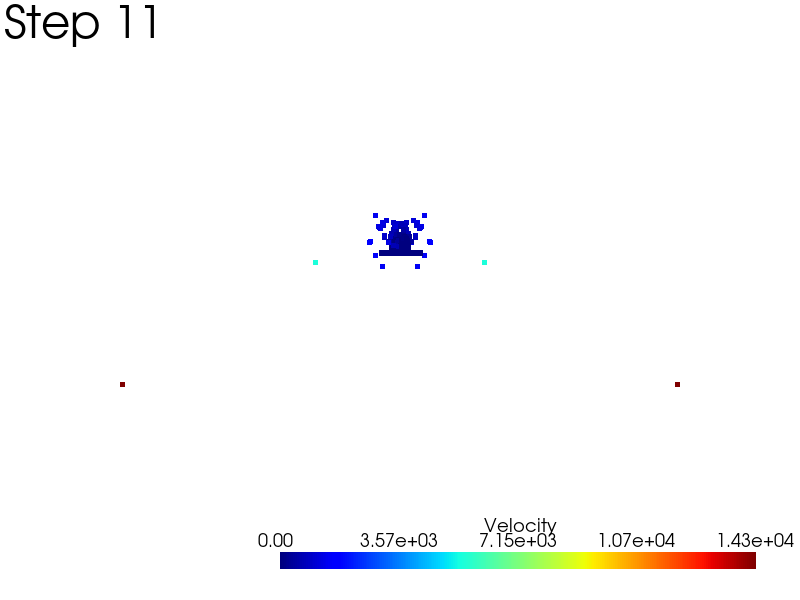
\includegraphics[width=0.8\textwidth]{image/step11.png}
%         \caption{液柱垮塌算例时刻 0.11}
%     \end{figure}
% \end{frame}

% \begin{frame}
%     \begin{figure}[H]
%         \includegraphics[width=0.8\textwidth]{image/step16.png}
%         \caption{液柱垮塌算例时刻 0.16}
%     \end{figure}
% \end{frame}

% \begin{frame}
%     \begin{figure}[H]
%         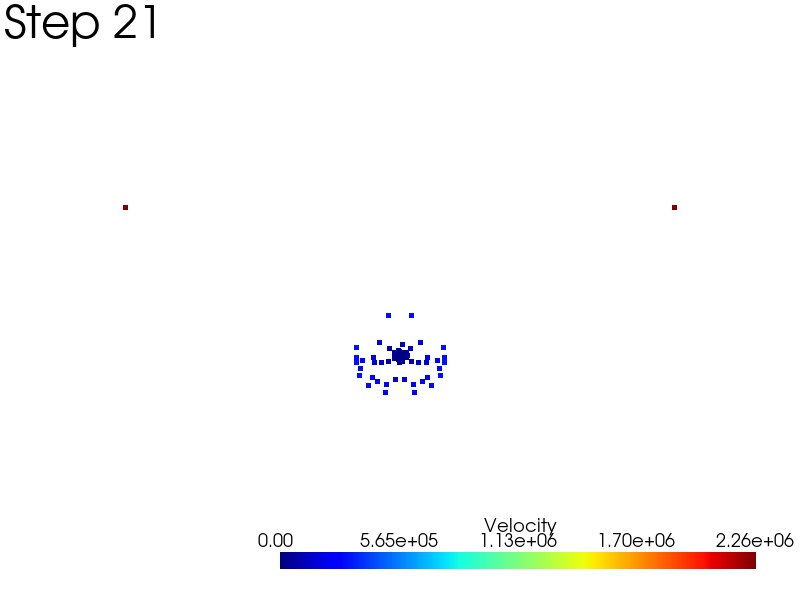
\includegraphics[width=0.8\textwidth]{image/step21.png}
%         \caption{液柱垮塌算例时刻 0.21}
%     \end{figure}
% \end{frame}

% \begin{frame}
%     \begin{figure}[H]
%         \includegraphics[width=0.8\textwidth]{image/step26.png}
%         \caption{液柱垮塌算例时刻 0.26}
%     \end{figure}
% \end{frame}

% \begin{frame}
%     \begin{figure}[H]
%         \includegraphics[width=0.6\textwidth]{image/step31.png}
%         \caption{液柱垮塌算例时刻 0.31}
%     \end{figure}

%     在第 0.31 时刻,液柱开始有点崩坏,
%     不清楚是数值格式中哪块出了问题。
%     目前可以肯定的是,
%     边界条件的处理是有问题的。
%     但在目前的程序结构下不知道采用什么别的格式好做一些。
% \end{frame}

\subsection{待完成的工作}

\begin{frame}
    \begin{itemize}
        \item 修复边界条件处理
        \item 检验核函数插值的正确性
        \item 尝试不可压缩的 SPH 数值格式
        \item 快速粒子搜索算法*(这点很重要,会影响到后面的工作)
    \end{itemize}
\end{frame}
% \section{SPH方法总结}


\subsection{SPH方法思想总结}

\begin{frame}
\begin{block}{一个比喻}
    在我简单的学习和阅读文献后,
    我认为SPH方法可以用一个形象的比喻来描述:
    假想我们在流体内细密地分布一种可以吸附流体的“吸水珠”,
    可以将附近核半径内的流体吸附到自己体内,
    形成一个理想质点。

    这样做的好处是,
    在求解方程时,
    这些吸水珠同时有如下两种性质:
    \begin{itemize}
        \item 质点性质:涉及到拉格朗日描述下刚体运动求解时,
        吸水珠呈现出质点的性质,即质点的质量、速度、位置等,
        此时流体质量都集中在这个质点上;
        \item 连续介质性质:在涉及到流体运动求解时,
        需要用到速度场的空间导数,用光滑核函数把这个吸水珠打开,
        将质量、能量、动量平摊在附近的空间上,
        此时这个质点呈现出连续介质的特性。
    \end{itemize}

    在传统流体求解中,
    流体网格的粗细对求解结果精度有很大影响,
    网格越粗,精度越低,但求解越快。
    同样的,SPH方法中,
    光滑核函数半径越大,精度越低,流体分布越稀疏,但求解更快。

    而因为SPH方法中对流体质点间并没有建立明确的几何拓扑关系,
    所以这些质点往往可以自由移动,
    从而可以很好地模拟流体的自由表面,
    避免传统方法中网格畸变或者重构网格的复杂过程。
\end{block}
\end{frame}

\subsection{SPH方法优缺点总结}

\begin{frame}

    SPH方法优点:
    \begin{itemize}
        \item 适用于自由表面流动
        \item 适用于高速撞击流动,不需要网格加密
        \item 适用于多相流动,用于解决流动中的相变问题
        \item 适用于流动中的破碎问题
        \item 适用于流动中的边界大变形问题
    \end{itemize}

    SPH方法缺点:
    \begin{itemize}
        \item 计算效率低,计算量大(没有连接信息,每步都需要计算两点间距)
        \item 很难评估算法的精度与收敛性,且各类光滑核函数的选取缺乏数学理论支撑
        \item 在某些情况下会出现数值空腔,或者粒子堆积现象
        \item 其流动后处理(如计算压力、速度场等)较为困难
        \item 若要与其他方法结合,缺乏边界处物理场信息交换的方法
    \end{itemize}

\end{frame}

% \section*{参考文献}
% \begin{frame}[allowframebreaks]
% 	\frametitle{\secname}
% 	\printbibliography[heading=none]
% \end{frame}

\end{document}